\chapter{Tabs-konceptet}
Udgangspunktet for beregningerne af en trådløs tjenestes fremkommelighed er en modellering af det effekt-tab, som radiosignalet har undervejs fra transmitteren til receiveren.
\section{ITU-R's koncept for tab over radio-forbindelser}
Et udbredt koncept ved anskuelse af transmissionstab er det, der allerede i 1951 første gang blev beskrevet af ITU i rekommendationen ITU-R P.341\cite{itur_p341-5}.

\begin{figure}[h]
	\centering
	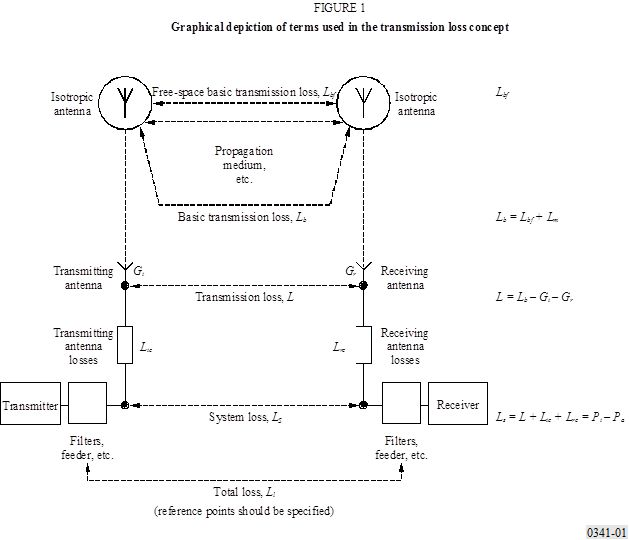
\includegraphics[width=0.8\textwidth]{figure/itur,P341-5,fig01.JPG}
	\caption{Rec. ITU.R P.341-5, figure 1, Graphical depiction of terms used in the transmission loss concept}
	\label{fig:tabskonceptet}
\end{figure}

Konceptet udmærker sig ved at isolere effekttab i radiokomponenter som antenner, filtre, bølgeledere, transceivere etc. fra effekttabet i radiosignalet på sin vej ind over landskabet.

Rekommendationen blev lavet i regnestokkenes tid, så alle effekter ($P$) er i $dB_m$ mens alle dæmpninger ($L$) og forstærkninger ($G$) er i $dB$.

\subsection{Systemtabet}
Det samlede tab i det viste koncept - kaldet ''\emph{systemtabet}'' - er det tab, signalet har fra transmitter til receiver, antennetab indbefattet. Modellen befatter sig ikke med tab i evt. filtre og bølgeledere. 

\begin{equation}
L_s =P_t -P_r
\end{equation}
hvor:
\begin{itemize}[]
 \item [$L_s$:] Tab for det samlede system
 \item [$P_t$:] Effekt afsendt af transmitteren (på udgangen af evt. filtre og bølgeledere) 
 \item [$P_r$:] Effekt modtaget af receiveren (på indgangen af evt. filtre og bølgeledere)
\end{itemize}

\subsection{Transmissionstabet}
\emph{Transmissionstabet ($L$)} er systemtabet uden tab i antennerne: 
\begin{equation}
L =L_s - L_{tx} - L_{rc}
\end{equation}
hvor:
\begin{itemize}[]
 \item [$L$:] Transmissionstabet
 \item [$L_s$:] Systemtabet 
 \item [$L_{tx}$:] Tab i senderantennen
 \item [$L_{rc}$:] Tab i modtageantennen
\end{itemize}

\subsection{Basistabet og antenneforstærkningen}
\emph{Basistabet ($L_b$)} er tabet over nogle teoretiske isotropiske (kugleformede) antenner, ækvivaleret med de faktiske antenner ved introduktionen af antenneforstærkningskonceptet: 
\begin{equation}
L_b =L + G_t + G_r
\end{equation}
hvor:
\begin{itemize}[]
	\item [$L_b$:] Basistabet 
	\item [$L$:] Transmissionstabet	
	\item [$G_t$:] Senderantennens forstærkning (i forhold til en isotrop antenne)
	\item [$G_r$:] Modtageantennens forstærkning (i forhold til en isotrop antenne)
\end{itemize}

Gevinsten ved indførelsen af antenneforstærkningskonceptet er, at man afkobler alle radiokomponenternes (incl. antennernes) karakteristika fra indflydelse på modellen for radiosignalets effekt-tab gennem luften over terrænet på sin vej fra sender til modtager. Definitionen på en antenne-forstærkning er givet i Annex 1, sektion 2 i ITU-R rekommendationen P.341\footnote{''The power gain of an antenna is defined as the ratio, usually expressed in decibels, of the power required at the input of a loss-free reference antenna to the power supplied to the input of the given antenna to produce, in a given direction, the same field strength or the same power flux-density at the same distance. When not specified otherwise, the gain refers to the direction of maximum radiation. The gain may be considered for a specified polarization.''} \cite{itur_p341-5}.

Sendendeeffekten ved den hypotetiske isotropiske sendeantenne er altså:
\begin{equation}
P_{it} = P_{t}+ G_t
\end{equation}
og modtageeffekten i den hypotetiske isotropiske modtageantenne bliver:
\begin{equation}
P_{ir} = P_{r}- G_r
\end{equation}
hvor:
\begin{itemize}[]
 \item [$P_{it}$:] Sendendeeffekten ud af den hypotetiske isotropiske sendeantenne 
 \item [$P_{t}$:] Sendendeeffekten ud af den faktiske sendeantenne
 \item [$P_{ir}$:] Modtageeeffekten ind i den hypotetiske isotropiske modtageantenne
 \item [$P_{r}$:] Modtageeeffekten ind i den faktiske modtageantenne
\end{itemize}
\FloatBarrier

\section{Longley-Rice's computer metode}
Et kendt eksempel på praktisk anvendelse af ITU's tabskoncept er den såkaldte Longley-Rice model -- også kaldet den \emph{I}rregulære \emph{T}erræn \emph{M}odel eller ITM. Denne model blev standard i U.S.A. allerede i 1965\cite{nbs-tn101}.

Longley og Rice havde kun 3 år efter - i 1968 - beskrevet en metode, hvorved man med en computer kan beregne tabet\cite{ntis-ad676874}.

Metoden dækker et stort dynamikområde. I tabel \ref{tab:lr-range} er området specificeret ud.

\begin{table}[h]
 \centering
 \begin{tabular}{ll}
   Parameter:                                   & Dynamikområde:\\
   \hline
   Frekvens                                     & 20 til 40.000 MHz\\
   Antennehøjde                                 & 0,5 til 3.000 m \\
   Distance                                     & 1 til 2.000 km \\
   Luftens brydningsindex (refraktivitet ($n$)) & 250 til 400 \\
 \end{tabular}
 \caption{Longley-Rice modellens dynamikområde}
 \label{tab:lr-range}
\end{table}
\FloatBarrier

\subsection{Input til den ITM modellen}



   
\subsection{Input til den ITM modellen}
I ITM modellen indgår parametre som beskrevet herunder:
\begin{description}
 \item [$d$] er forskellige afstande (f.eks. afstanden mellem sender og modtager). Alle afstande angives i kilometer.
 \item [$h$] er højder (f.eks. en antennes højde over jordoverfladen). 
 \item [$k$] er radiosignalets centerfrekvens ($f$) målt i radianer ($k = 2 \pi f$)
 \item [$\Delta h$] er en parameter, der angiver, hvor ujævnt landskabet er.
 \item [$N$] er luftens brydningsindex.
 \item [$a$] er en kugles radius (f.eks. jordens radius).
% \item [$Z$] er impedans (f.eks. luftens impedans ved jordens overflade).
\end{description}

\subsubsection{Radiobølgens udbredelse ($d$)}
$d$ er den afstand radiobølgen tilbagelægger. På en Line-of-Sight radiokæde har $d$ én værdi. Det er afstanden mellem sende- og modtageantennen. For rundspredningstjenester som GSM, radiofoni og lignende har $d$ lige så mange værdier som der er punkter i tjenestens dækningsområde.   

\subsubsection{Antennens højde over jorden ($h_g$)}
$h$ er en given antennes højde over jorden. ITM-modellen skelner mellem antennens faktiske højde ($h_g$) over terrænnet, også kaldet antennens strukturelle højde, og antennens effektive højde ($h_e$) over jorden, der simpelt sagt er antennens højde over terrænets gennemsnitshøjde over radiobølgens udbredelsesområde. 

\subsubsection{Radiosignalets centerfrekvens målt i radianer ($k$)}
Radiosignalets centerfrekvens målt i radianer er givet ved:
\begin{equation}
k = 2 \pi f
\end{equation}
hvor $f$ er radiosignalets centerfrekvens. Iøvrigt gælder, at:
\begin{equation}
c = \lambda f
\end{equation}
hvor $c$ er lysets hastighed i luft (i omegnen af $2,997 \cdot 10^8$ m/s) og $\lambda$ er centerfrekvensens bølgelængde.

\subsubsection{Luftens brydningsindex ($N$)}\label{N}
Luftens brydning alias radiosignalets refraktivitet ændrer radiosignalets retning på sin rejse, så signalet typisk krummer. Dette fænomen afhænger af forskellige variabler som luftens tryk, sammensætning, renhed og fugtighed. Der er i ITU-R's rekommendation P.453 \cite{itur_p453-11} forsøgt kortlagt nogle målinger og givet nogle modeller for luftens middelbrydning rundt om i verden. I ITM-modellen bruges målte og kortlagte middelbrydningsværdier ved jordens overflade ($N_s$) som udgangspunkt. Der ønskes en værdi for $N_s$, der passer best muligt til virkeligheden, men det virkelige brydningsindex ($N$) varierer som nævnt med vejret.
\par
Både i ITU-R's rekommendation P.453-11 og i Longley-Rice's ITM gives en formel, hvor $N_s$ udregnes ud fra: 
\begin{description}
	\item[$N_0$,] der er "minimum måneds-middelværdier" af $N_s$ "reduceret til havets overflade", og
	\item[$h_s$,] der for Line-of-Sight forbindelser er højden i [km] over havet (Mean Sea Level) ved den laveste antenne.
\end{description}
ITU-R P.453-11 giver den empiriske formel:
\begin{equation}
N_s = N_0 \cdot e^{(-h_s / h_0)}
\end{equation}
og nævner at $h_0$ måske kan være $7,35$ [km]. Longley og Rice giver formlen:
\begin{equation}
N_s = N_0 \cdot e^{(-0,1057 \cdot h_s)}
\end{equation}
og uddyber, hvorledes de ud fra måledata er kommet frem til denne tilnærmelsesformel (se side 4-1 i \cite{nbs-tn101}). At omregningsformlerne er forskellige i de to kilder indikerer, at modellerne bygger på statistik og ikke eksakt videnskab. I figur \ref{fig:N0} er vist et eksempel på et verdenskort visende $N_0$. I sagens natur bør man være kritisk ved anvendelsen af kort som disse og forsøge altid at finde de nyeste målinger.

\begin{figure}[h]
 \centering
 \includegraphics[width=0.8\textwidth]{figure/itur,P453,fig01.JPG}
 \caption{Rec. ITU.R P.553-11, FIGURE 1, Monthly mean values of N0: February}
 \label{fig:N0}
\end{figure}
 
\subsubsection{Jordens effektive radius ($a$) og krumning ($\gamma_e$)}
Hvis jorden var helt rund ville jordens krumning være den reciprokke værdi af jordens radius, og hvis luften ikke brød et radiosignal ville man i denne ideelle verden have en retlinet signaludbredelse. Jordens effektive radius ($a$) er den hypotetiske radius, der retter et radiosignals krumme bane gennem luften ud til en ret bane. Jordens effektive krumning ($\gamma_e$) er den reciprokke værdi af jordens effektive radius. Disse to parametre afhænger altså af luftens brydning.
\par
Uagtet jorden ikke er rund sætter Longley og Rice jordens "faktiske" radius til 6370 km og udregner herefter jordens effektive radius ($a$) i enheden [km] som:

\begin{equation}
a = 6370 \cdot \frac{1}{1-0,04665 \cdot e^{0.005577 \cdot N_s}}
\end{equation}
hvor $N_s$ er luftens middel-brydningsindex ved jordens overflade som beskrevet ovenfor. ITU-R P.453-11 har naturligvis en anden formel her, som jeg ikke vil uddybe nærmere. Jordens effektive radius ligger på omkring $4/3$ af jordens ''faktiske'' radius.

\subsection{Den glatte kurve gennem terrænet}
Der laves en cirkelbue gennem terrænet mellem sende- og modtageantennen, således at cirkelbuen skærer gennem terrænnet under den laveste antennes mastefod. 

\subsubsection{Matematisk beskrivelse af terrænet ($\Delta h(d)$)}
Terrænets beskaffenhed tages ind i Longley-Rice modellen med blandt andet parameteren $\Delta h(d)$, som er middelværdien af højdeforskellene i terrænet mellem sende- og modtage-antennerne. Matematisk kan det skrives som:

\begin{equation}
\Delta h(d) = \sum\limits_{n=1}^N \frac{\Delta h_n}{\Delta d_n} \xrightarrow {N\rightarrow \infty} \Delta h
\end{equation}
hvor:
\begin{itemize}
	\item [$\Delta h_n = h_n - h_{n-1}$:] er terrænets højdetilvækst på positionen for den $n$'te måling [m]. 
	\item [$\Delta d_n = d_n - d_{n-1}$:] er afstanden mellem den $n$'te og den $n-1$'te måling [km]. 
\end{itemize}

\FloatBarrier